\documentclass{article}

\usepackage{graphicx}
\usepackage{subfig}
\usepackage{amsmath}
%\usepackage{amsmath,rotating}

\title{Three-dimensional Taylor Green}

\date{}

\begin{document}

\maketitle

\section{Introduction}
The Taylor-Green vortex at a Reynolds number of 1600 is a configuration 
commonly studied flow that captures elements of rudimental turbulence generation and 
decay~\cite{taylorGreen}. This canonical case serves as a testbed for a high-order workshop~\cite{hillewaert2012}
where various schemes can be compared and contrasted. 
Unstructured, low-Mach numerical approaches were presented in~\cite{domino2019} using a series of 
homogenous topologies consisting of the following: Hex8, Hex27, Tet4, Pyramid5, and Wedge6 where
convergence and relative accuracy was assessed relative to the reference direct numerical simulation (DNS).

The Taylor-Green flow regime is marked by three phases that are described as the following: Phase 1, viscous effects 
with small-scale laminar and organized structures are found; Phase 2, viscous (diffusion) effects 
dominating with accompanying stretching of vortex lines, and Phase 3, a break-up and is nearly 
isotropic in nature. Generally, for this simulation study, an explicit LES sub-grid stress model 
is omitted.  

The initial condition for the three-dimensional flow field is as follows:
%
\begin{eqnarray}
u_x &=& u_o sin(\frac{x}{L})cos(\frac{y}{L})cos(\frac{z}{L}), \nonumber \\
u_y &=& -u_o cos(\frac{x}{L})sin(\frac{y}{L})cos(\frac{z}{L}), \nonumber \\
u_z &=& 0, \nonumber \\
p &=& p_o + \frac{\rho_o u_o^2}{16}\left(cos(\frac{2x}{L}) + cos(\frac{2y}{L})\right)\left(cos(\frac{2z}{L})+2\right).
\end{eqnarray}

The quantities of interest (QoIs) for this simulation study are the temporal evolution of the kinetic energy, $E_k$, that
is integrated over the full domain at each time step, the integrated dissipation rate as a function of time, and the temporal enstrophy
response. The energy-based dissipation rate is given by $\epsilon_1 = -\frac{dE_k}{dt}$. 
The integrated enstrophy, $\zeta$ is defined by (in a low-Mach flow), $\epsilon_2 = \frac{2 \mu}{\rho_o} \zeta$,
where,

\begin{equation}
\zeta = \frac{1}{\rho_o V} \int_\Omega \frac{1}{2}\rho \omega_k \omega_k d\Omega.
\end{equation}
%
For more details, see~\cite{bullAndJameson2015}.

\section{Domain}
The simulation is run in a periodic square box of $-\pi L \leq x,y,z \leq \pi L$ with $L$ equal to unity. The simulation
is allowed to evolve from this initial condition over 20 characteristic convection time scales (defined 
by $t_c = \frac{L}{u_o}$). For this configuration, peak dissipation occurs at approximately $8t_c$.

\subsection{Simulation Specification and Sample Results}
A sample Q-criterion set of images for a Taylor-Green Re 1600 image appearing in~\cite{domino2019} is shown in 
Figure~\ref{fig:q}, while the set of converged results in this same paper are shown in Figure~\ref{fig:ek}.

\begin{figure}[!htbp]
  \centering
  {
   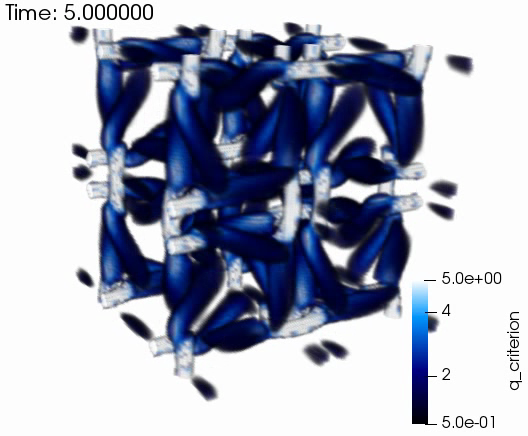
\includegraphics[height=1.5in]{images/tg_5s.png}
  }
  {
   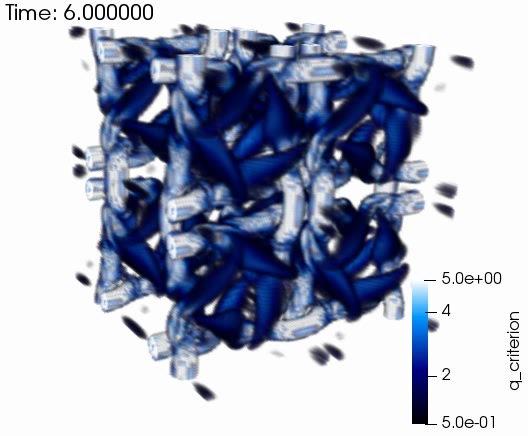
\includegraphics[height=1.5in]{images/tg_6s.png}
  } \\
  {
   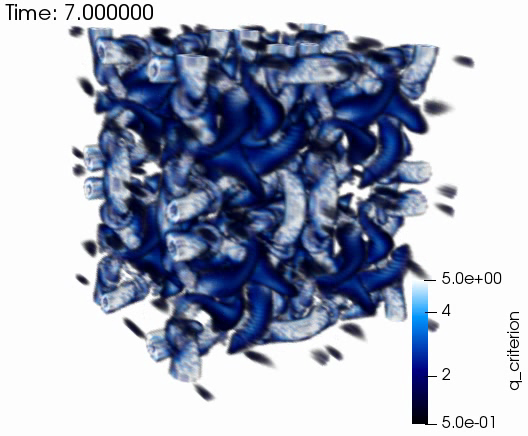
\includegraphics[height=1.5in]{images/tg_7s.png}
  }
  {
   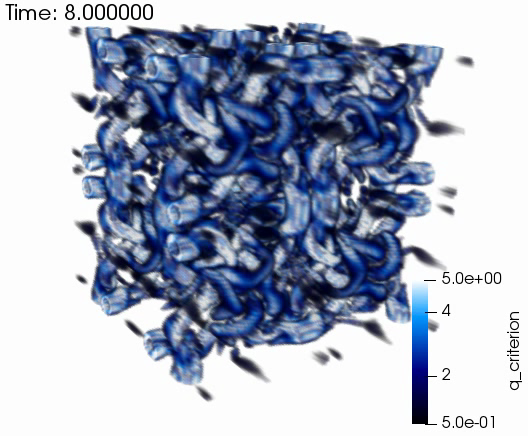
\includegraphics[height=1.5in]{images/tg_8s.png}
  }
  \caption{Three-dimensional Q-criterion volume rendered Taylor-Green representative time series at 5, 6, 7, and 8 seconds.}
  \label{fig:q}
\end{figure}

\begin{figure}[!htbp]
  \centering
  {
   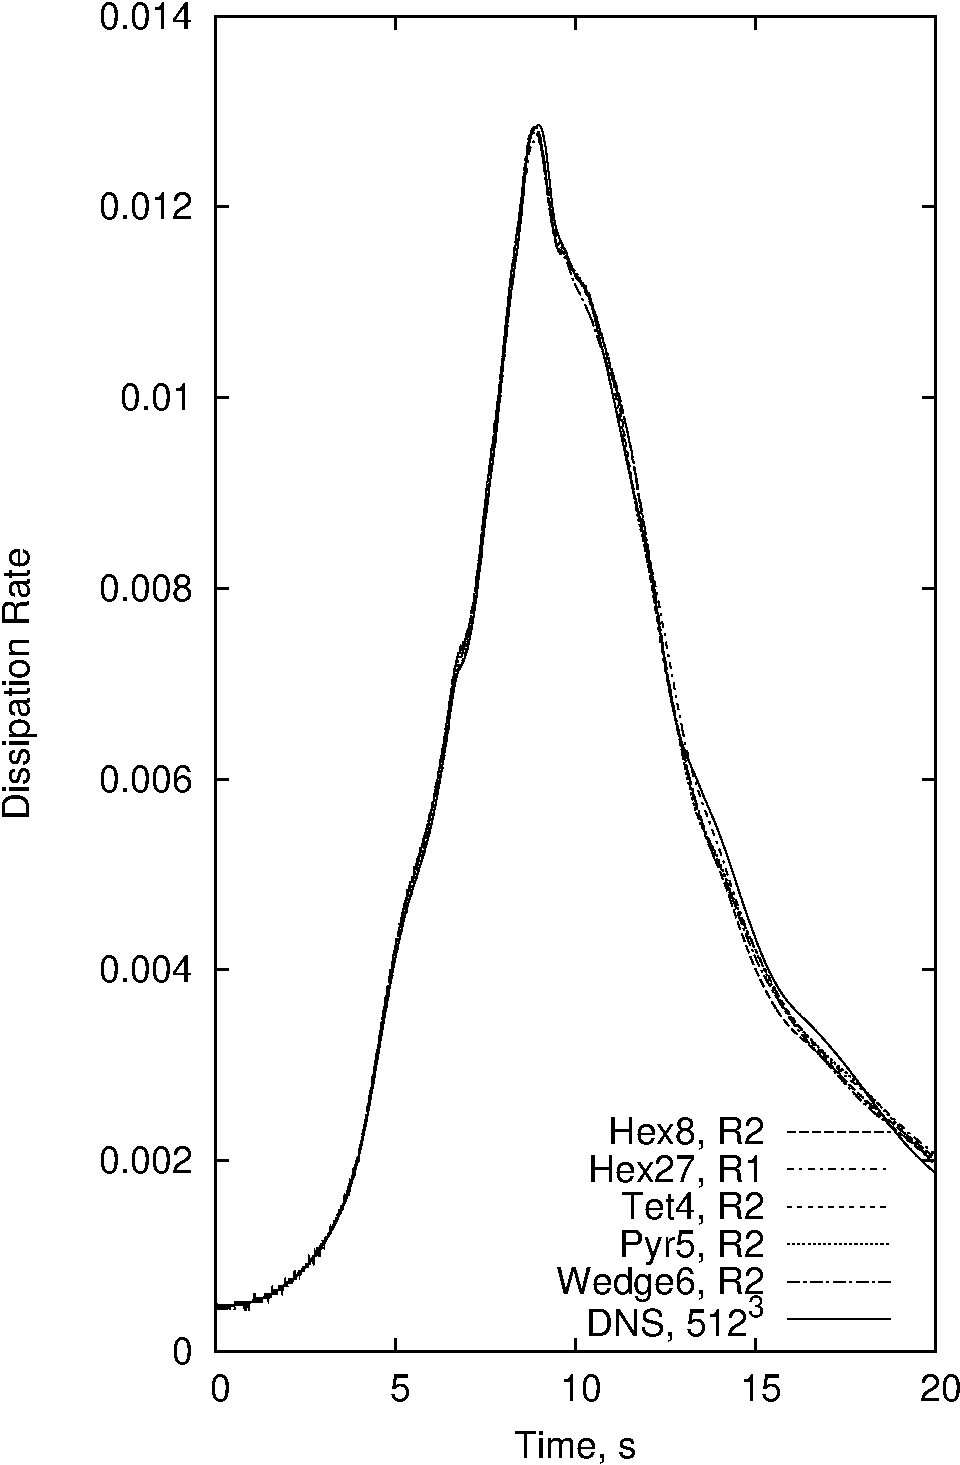
\includegraphics[height=4.0in]{images/tg_diss_hex8_tet4_pyr5_wedge6_R2_CU-crop.pdf}
  }
  \caption{Turbulence dissipation rate temporal plot for the series of mesh refinements in~\cite{domino2019}. In this
study, the baseline (R0) Hex8 mesh spacing of $\frac{2\pi}{100 L}$, i.e., $100^3$ elements was used.}
  \label{fig:ek}
\end{figure}

\subsection{Meshes}
The set of meshes provided in the /mesh directory are as follows:

\begin{itemize}
	\item 3d\_hex8\_taylor\_green\_0p2.g (Hex8 topology using 0.2 mesh spacing)
	\item 3d\_tet4\_taylor\_green\_0p2.g (Tet4 topology using 0.2 mesh spacing)
	\item 3d\_tet4\_taylor\_green\_0p4.g (Tet4 topology using 0.4 mesh spacing)
\end{itemize}
The ``0p4'' mesh can be useful for trouble shooting the monolithic  code implementation. Note that most peer-reviewed results 
appearing in the open literature exercise meshes that, even for a coarsest mesh spacing reported, are far more refined than 
the meshes provided in this study. However, the prime motivation for this exercise is to learn more about fully implicit solver approaches
in the low-Mach limit.

\section{Equation Set}
The variable-density low-Mach equation set is defined by the continuity and momentum equation, here shown in
integral form,

\begin{align}
 \int  \frac {\partial \rho }{\partial t} dV + \int \rho \hat{u}_j n_j dS = 0,
\label{eq:contEq}
\end{align} 

\begin{align}
\int  \frac {\partial \rho u_i }{\partial t} dV + \int \rho \hat{u}_j u_i n_j dS 
-\int 2 \mu S^*_{ij} n_j dS = \int P \delta_{ij} n_j dS
\label{eq:momEq}
\end{align}
%
In the above equation, $\rho$ is the fluid density and $u_i$ is the fluid velocity, while
the traceless rate-of-strain tensor is defined as
\begin{align}
S^*_{ij}  = S_{ij} - \frac{1}{3} \delta_{ij} S_{kk} \nonumber
		     = S_{ij} - \frac{1}{3} \frac{\partial  u_k }{\partial x_k}\delta_{ij}.
\end{align}
In a low-Mach flow, the above pressure, $P$, is the perturbation about the thermodynamic
pressure, $P^{th}$. We also note that the form shown above includes pressure stabilization
embedded in the special velocity, $\hat{u}_j$, whose form can be written as,

\begin{align}
\rho \hat{u}_j = \rho u_j -\frac{\Delta t}{\gamma_1}\left(\frac{\partial P}{\partial x_j} - G_j P\right),
\end{align}
where the projected nodal gradient, $G_jP$ is obtained though the following equation:
\begin{align}
\int G_j P dV - \int P n_j dS = 0.
\end{align}

When using higher-order approaches, and to retain design-order accuracy, $G_jP$ must be computed
using the consistent mass matrix, while using mass-lumping, yields,
\begin{align}
G_j P = \frac{\int P n_j dS}{\int dV}.
\end{align}
As captured in the tutorial notes, this Rhie-Chow-like form~\cite{rhieChow1983} can be shown to be an algebraic manipulation of the
assembled momentum system to approximate the fine-scale momentum equation (see also~\cite{martinez2017}). In general, the
states associated with the projected nodal gradient can drastically improve nonlinear convergence as can the time scale chosen 
(above, the simulation time step, $\Delta t$ is used). In most cases, the projected nodal gradient is lagged by one iteration since inclusion of this
equation can increase the implicitly coupled system. As such, quadratic nonlinear convergence
within a time step can be affected when using this lagged approach since sensitivities to the fully coupled system are missing. However, 
choosing this value to be the state $n$ quantity can improve convergence, while influencing time accuracy. 

There are also instances where the effect of pressure stabilization is not propagated to the momentum equation and, if in use, any other transport equation, e.g.,
mass fraction, enthalpy, etc. In the simplest form, $\rho \hat{u}_j = \rho u_j$, while in Charnyi et al.~\cite{charnyi2017}, the termed energy, momentum and angular momentum (EMA) method is described. 

\section{Discussion Points}

There are several interesting activities associated with this sample case including
the points captured below. 

\begin{itemize}
	\item Document the appropriate equations for this conceptual model problem. Feel free to enforce the incompressible
          	constraint since this approach simplifies the continuity equation and both the momentum time and viscous term.
	\item Run the pressure projection input file (modified to run at least 20 seconds), while post-processing the integrated 
		kinetic energy and dissipation plots. For the reference DNS of~\cite{hillewaert2012}, see the ``/data''  directory. In recent versions of Nalu, the 
		log file for the simulation will contain values such as "sum(vol), sum(ke*vol), mean(ke)" that represents the total volume, integrated kinetic energy, 
		and mean kinetic energy of the system at each converged time step. Use both the 0p2 Hex8 and Tet4 mesh in this study, while visualizing the flow field.
		Comment on the kinetic energy and dissipation rate time history for each topology relative to each other and the DNS. Note that you will need to 
		differentiate the kinetic energy data in time to obtain the dissipation rate plot. Most plotting packages, e.g., Matlab, Tecplot, etc., support this post-processing step.
        \item Implement an interior monolithic momentum and continuity kernel that captures the equation contributions identified 
        		in the above first step. In fact, this kernel should look very much like a combination of the segregated continuity (ContinuityAdvElemKernel) 
          	and momentum (MomentumAdvDiffElemKernel and MomentumMassElemKernel) classes, while noting that the total 
		size of the new monolithic system represented in your new kernel is now $nDim+1$. This differs from the segregated kernels 
		where momentum is size $nDim$ and continuity is unity in size. In the LowMachMonolithicEquationSystem class, a single kernel contribution is expected 
		by the name of: 
			\begin{itemize}
				\item uvwp\_time\_advection\_diffusion (a consistent-mass kernel) or,
				\item uvwp\_lumped\_time\_advection\_diffusion (a lumped-mass kernel)
			\end{itemize}
		A purely diagonal monolithic system can be obtained simply by copying the code from the segregated Continuity and Momentum
		kernels and by modifying the total size of the matrix system. As a hint, the easiest approach may be to use the 0, 1, and 2 memory location for the momentum
		contribution, and the "AlgTraits::nDim\_" entry for continuity. Include the code base in the report prepared as an appendix item. Of coarse, the objective
		of this laboratory is to include the cross Jacobian entries, e.g., $\frac{\partial C}{\partial u_j}$ and $\frac{\partial U_j}{\partial P}$, where $C$ and $U_j$ represent the
		continuity and momentum equation. The 0p4 Tet4 mesh may be useful for debugging.
	\item Run the monolithic kernel that you have implemented and compare nonlinear convergence between the production pressure projection scheme and your 
		monolithic kernel. Comment on overall speed to reach the end simulation time.
	\item Explore the usage of pressure stabilization in the momentum mass flow rate expression, in addition 
		to using the "old" values for the momentum and projected nodal pressure gradient field. You may also explore other forms of the
		advection form, i.e., EMA, although do not worry about implementing any upwind or residual-based operator to manage advection stabilization.
	\item Compare and contrast the simulation timings between the pressure projection and monolithic implementation at varying nonlinear tolernaces. 
	\item $Optional, not-required:$ As time permits, perform any mesh refinement and comment on the sensitivity of the QoIs.
	\item $Optional, not-required:$ Perform any appropriate code verification using, for example, the convecting Taylor Vortex analytical solution
		on a periodic domain using your newly coded monolithic implementation.		
	\item $Optional, not-required:$ Explore other forms of the advection operator, i.e., EMA and report findings as compared to the advection form shown in this report.
	\item $Optional, not-required:$ Implement various upwind approaches via the usage of the nodal field "dudx".
	\item $Optional, not-required:$ Implement a residual-based stabilization approach and comment on how this usage affects both convergence and QoIs.
	\item $Optional, not-required:$ Perform mesh refinement and capture results compared to the DNS reference solution.
\end{itemize}


\bibliographystyle{unsrt}
\bibliography{3d_tet4_taylor_green_0p2}

\end{document}
